\documentclass[fleqn]{beamer}
\beamertemplatenavigationsymbolsempty

\usepackage[T1]{fontenc}
\usepackage[utf8]{inputenc}

\usepackage{amsmath,amssymb}
\usepackage{nccmath}
\usepackage{graphicx}
\usepackage{mathptmx}
\usepackage{mathtools}
\usepackage{subcaption}
\usepackage{amsthm}
\usepackage{tikz}
\usepackage{enumitem}
%\usepackage[colorlinks=true,naturalnames=true,plainpages=false,pdfpagelabels=true]{hyperref}
\usetikzlibrary{patterns,decorations.pathmorphing,positioning, arrows, chains}

\newcommand{\tabitem}{%
  \usebeamertemplate{itemize item}\hspace*{\labelsep}}

\usepackage[backend=biber, sorting=none]{biblatex}
\addbibresource{uni.bib}

\setbeamertemplate{endpage}{%
    \begin{frame}
        \centering
        \Large \emph{Thank you for listening!}
    \end{frame}
}

\AtEndDocument{\usebeamertemplate{endpage}}

% vertical separator macro
\newcommand{\vsep}{
  \column{0.0\textwidth}
    \begin{tikzpicture}
      \draw[very thick,black!10] (0,0) -- (0,7.3);
    \end{tikzpicture}
}
\setlength{\mathindent}{0pt}

% Beamer theme
\usetheme{UniVienna}
\usefonttheme[onlysmall]{structurebold}
\mode<presentation>
\setbeamercovered{transparent=10}

\title
{Mathematical Modeling of Water-Wave Problems}
\subtitle{Applied PDE Seminar}
%\author[Popović Milutin]
%{Popović Milutin \inst{1}\\[1ex] {\small supervisor\inst{1,2}}

\author[Popović Milutin]{Popović Milutin\\[10mm]{\small Supervisor: Sabine Hittmeir}}
\date{29. June 2022}

\begin{document}
    \begin{frame}
        \titlepage
        \nocite{johnson_1997}
        \nocite{vallis_2017}
        \nocite{constantin_tsunami}
        \nocite{rupert_2009}
        \nocite{mathe-physik}
    \end{frame}


    \begin{frame}
        \frametitle{Fluid Description}
        \begin{columns}[T]
            \column{0.34\textwidth}
            \hspace{50cm}

            The fluid is described by
            \begin{itemize}
                \item[$\circ$] Fluid density\\ $\rho(\vec{x}, t)$
                \item[$\circ$] Velocity Field\\ $\vec{u}(\vec{x}, t) = (u, v,
                    w)$
            \end{itemize}
            \column{0.57\textwidth}

            \begin{figure}[H]
                \centering
                \caption{Control volume of the fluid}
              \begin{tikzpicture}[>=latex,scale=1, xscale=1, opacity=.8]
            % second sphere
                \begin{scope}[rotate=10, xscale=3, yscale=2, shift={(2.3,-0.2)}]
                  \coordinate (O) at (0,0);
                  \shade[ball color=gray!10!] (0,0) coordinate(Hp) circle (1) ;

                  \draw[thick] (O) circle (1);
                  \draw[rotate=5] (O) ellipse (1cm and 0.66cm);
                  \draw[rotate=90] (O) ellipse (1cm and 0.33cm);
            \node[circle, fill=black, inner sep=1pt] at (0.15, 0.25) {} ;
            \draw[-latex, thick] (0.15, 0.25) -- (1, 1) ;
                  \node[right] at (1, 1) {$\vec{u}(\vec{x}, t)$};

                  \node[] at (O) {$V$};
                  \node[] at (0.55, -0.25) {$\rho(\vec{x}, t)$};

                  \draw[-] (0.76, -0.66) -- (1.2, -0.7);
                  \node[right] at (1.2, -0.7) {$S$};

                  \draw[-latex, thick] (-0.25, -0.65) -- (-1, -1);
                  \node[left] at (-1, -1) {$\vec{n}$};
                \end{scope}
              \end{tikzpicture}
            \end{figure}
        \end{columns}
    \end{frame}

    \begin{frame}
        \frametitle{Mass Conservation}
        \begin{itemize}
            \item[$\circ$] Mass:
            \begin{align}
                \hspace{0.3\linewidth}
                m(t) = \int_V \rho(\vec{x}, t)\ dV \nonumber
            \end{align}
        \item[$\circ$] Rate of change:
            \begin{align}
                \hspace{0.15\linewidth}
                \int_V \frac{\partial \rho(\vec{x}, t)}{\partial t}\ dV = \frac{dm}{dt} =
                -\int_{S} \rho(\vec{x}, t) \vec{u}\cdot\vec{n}\ dS\nonumber
            \end{align}
        \item[$\circ$] Use Gauss's law to get the \textbf{Equation of Mass
            conservation}
            \begin{align}
                \hspace{0.3\linewidth} \frac{\partial \rho}{\partial t}
                +\nabla \cdot (\rho \vec{u}) =
                0 \nonumber
            \end{align}
        \end{itemize}
    \end{frame}

    \begin{frame}
        \frametitle{Euler's Equation of Motion}
        \centering
        $\rightarrow$ Apply Newton's second law to the Fluid
        \begin{columns}
            \column{0.4\textwidth}
            \begin{block}{\centering\textbf{Body Force}}
                \centering
                $\vec{F} = (0, 0, -g)$
            \end{block}
            \column{0.4\textwidth}
            \begin{block}{\centering\textbf{Local/Short-range Force}}
                \centering
                Stress tensor\\
                For inviscid fluid: $P(\vec{x},t)$
            \end{block}
        \end{columns}
        \begin{align}
            \hspace{0.3\linewidth}\Rightarrow\int_V \rho \frac{D\vec{u}}{Dt}\ dV =
            \int_V \left( \rho \vec{F} - \nabla P \right)\ dV\nonumber
        \end{align}
        \centering
        $\rightarrow$ Leads us to \textbf{Euler's Equation of Motion}
        \begin{align}
            \hspace{0.4\linewidth} \frac{D\vec{u}}{Dt} =-
            \frac{1}{\rho}\nabla P + \vec{F}  \nonumber
        \end{align}
    \end{frame}

    \begin{frame}
        \frametitle{Vorticity}
        \begin{columns}
            \column{0.4\textwidth}
            \begin{block}{\centering\textbf{Vorticity}}
                \centering
                $\vec{\omega} = \nabla \times \vec{u}$
            \end{block}
            \column{0.4\textwidth}
            \begin{block}{\centering\textbf{Irrotational Flow}}
                \centering
                $\vec{\omega} = 0$
            \end{block}
        \end{columns}
        \vspace{0.5cm}

        \centering $\rightarrow$ Vorticity pops up in the acceleration of
        the fluid particles
        \begin{align}
            \hspace{0.25\linewidth}
            \frac{D\vec{u}}{Dt} = \frac{\partial \vec{u}}{\partial t}+
            \nabla \left( \frac{1}{2} \vec{u} \cdot \vec{u}\right)  - \left(
            \vec{u}\times \vec{\omega}  \right)\nonumber
        \end{align}

        \centering $\rightarrow$ We can incorporate vorticity into Euler's
        Equation of Motion
        \begin{align}
            \hspace{0.25\linewidth}\frac{\partial \vec{u}}{\partial t} + \nabla\left(
            \frac{1}{2}\vec{u}\cdot\vec{u} + \frac{P}{\rho} + \Omega \right)
            = \vec{u} \times \vec{\omega} \nonumber
        \end{align}
    \end{frame}

    \begin{frame}
        \frametitle{Perfect Fluid}
        \begin{itemize}
            \item \textbf{inviscid} $\mu = 0$
            \item \textbf{incompressible} $\rho = \text{const}.$, then
                $\nabla \vec{u} = 0$
        \end{itemize}

    \end{frame}

    \begin{frame}
        \frametitle{Boundary Conditions for Water Waves}
        \begin{center}
        \begin{tabular}{@{}l@{}}
        \tabitem \textbf{Kinematic Condition}: Fluid particles at the
            surface\\
        \tabitem \textbf{Dynamic Condition}: Atmospheric Pressure on
            the surface\\
        \tabitem \textbf{Bottom Condition}: Rigid and fixed bottom\\
        \tabitem (\textbf{Integrated Mass Condition}): Combination
        \end{tabular}
        \end{center}
   \end{frame}

    \begin{frame}
        \frametitle{Nondimensionalisation}
        \begin{center}
        \begin{tabular}{@{}l@{}}
                \tabitem $h_0$ for the typical water depth\\
                \tabitem $\lambda$ for the typical wavelength\\
                \tabitem $\sqrt{g h_0}$ velocity scale of waves in
                $(x, y)$\\
                \tabitem $\frac{\lambda}{\sqrt{g h_0}}$ time scale
                of wave propagation\\
                \tabitem $\frac{h_0 \sqrt{g h_0} }{\lambda}$ velocity scale in $z$
        \end{tabular}
        \end{center}
        \centering
        $\rightarrow$ \textbf{Shallowness parameter} $\delta =
        \frac{h_0}{\lambda}$
        \\
        \centering
        $\rightarrow$ \textbf{Amplitude parameter}
        $\varepsilon=\frac{a}{h_0}$
    \end{frame}

    \begin{frame}
        \frametitle{Nondimensionalisation}
        $\rightarrow$ Nondimensionalisation
        \begin{ceqn}
        \begin{align}
            &x \rightarrow\ \lambda x, \quad u \rightarrow \sqrt{gh_0} u,
            \nonumber \\
              &y \rightarrow\ \lambda y, \quad v \rightarrow \sqrt{gh_0} v, \qquad
              t\rightarrow \frac{\lambda}{\sqrt{gh_0}}t,\nonumber\\
              &z \rightarrow\ h_0 z, \quad w \rightarrow
            \frac{h_0\sqrt{gh_0}}{\lambda} w.\nonumber
        \end{align}
        \end{ceqn}
        \centering
        $\rightarrow$ Top and Bottom conditions
        \begin{ceqn}
        \begin{align}
        h = h_0 + a \eta(\vec{x}_\perp,t), \qquad  b \rightarrow h_0
        b(\vec{x}_\perp, t)\nonumber
        \end{align}
        \end{ceqn}
        \centering
        $\rightarrow$ Rewrite Pressure
        \begin{ceqn}
        \begin{align}
            P = P_a + \rho g(h_0 -z) + \rho g h_0 p(\vec{x})  \nonumber
        \end{align}
        \end{ceqn}
    \end{frame}

    \begin{frame}
        \frametitle{Scaling}
        \centering
        $\rightarrow$ $w$, $p$ and the free surface $z$ are $\propto$
        $\varepsilon$, leading to the scaling
        \begin{ceqn}
            \begin{align}
                p \rightarrow \varepsilon p, \quad w \rightarrow \varepsilon w, \quad
                \vec{u}_\perp \rightarrow \varepsilon
                \vec{u}_\perp\nonumber
            \end{align}
        \end{ceqn}
        \end{frame}

    \begin{frame}
        \frametitle{Results}
        \centering
        $\rightarrow$ Nondimensionalized Euler's Equation of motion
        \begin{ceqn}
        \begin{align}
            \frac{Du}{Dt} = - p_x \quad
            &\frac{Dv}{Dt} = - p_y \quad
            \delta^2\frac{Dw}{Dt} = - p_z \nonumber\\
            \nonumber\\
            &\nabla \cdot \vec{u}  = 0\nonumber
        \end{align}
        \end{ceqn}
        \centering
        $\rightarrow$ With boundary conditions
        \begin{ceqn}
        \begin{align}
            \begin{drcases}
            p = \eta - \frac{\delta^2\varepsilon h_0}{\lambda^2} \frac{W_e}{R}\\
            w = \frac{1}{\varepsilon}\eta_t + (\mathbf{u}_\perp \nabla_\perp)\eta
            \end{drcases} \quad
            \text{on}\;\; z = 1+\varepsilon\eta\\
            w =\frac{1}{\varepsilon}b_t + (\mathbf{u}_\perp \nabla_\perp)b \quad
            \text{on}\;\; z=b
        \end{align}
        \end{ceqn}
    \end{frame}

    \begin{frame}
        \frametitle{History of the Soliton}
        \begin{itemize}
        \item[$\circ$] John Scott Russell discovered the solitary wave in 1834,
            firstly calling it the \textbf{wave of translation}
        \item[$\circ$] a \textbf{soliton} is a solitary wave that resists
            dispersion, maintaining its shape while it propagates at constant
            velocity\\
        \end{itemize}
    \end{frame}

    \begin{frame}
        \frametitle{Korteweg-de Vries equation (KdV)}
        Korteweg-de Vries equation: nonlinear PDE
        \begin{ceqn}
        \begin{align}
            \eta_t + 6K \eta \eta_{x} + \eta_{x x x} = 0\nonumber
        \end{align}
        \end{ceqn}
        With Solution
        \begin{ceqn}
        \begin{align}
            \eta(x, t) = 2c^2 \text{sech}^2\Big( c
            \left(x - 4c^2t\right)  \Big)\nonumber
        \end{align}
        \end{ceqn}
    \end{frame}

    \begin{frame}
        \frametitle{KdV Regime}
        \begin{itemize}
            \item[$1$)]  The KdV equation arises in the $\varepsilon = O(\delta^2)$
            \item[$2$)] by rescaling $\delta$ in favor of $\varepsilon$ in
                Euler's Equations of motion
            \item[$3$)] going into the frame of the moving wave $(\xi = x- t, \tau = \varepsilon t)$
            \item[$4$)] conducting an Asymptotic expansion of $u , w, p$ and $\eta$.
            \item[$5$)] KdV equation is present in the $\varepsilon^1$ term
        \end{itemize}
    \end{frame}

    \begin{frame}
        \frametitle{2004 Tsunami: Description}

        \begin{figure}[htpb]
            \centering
            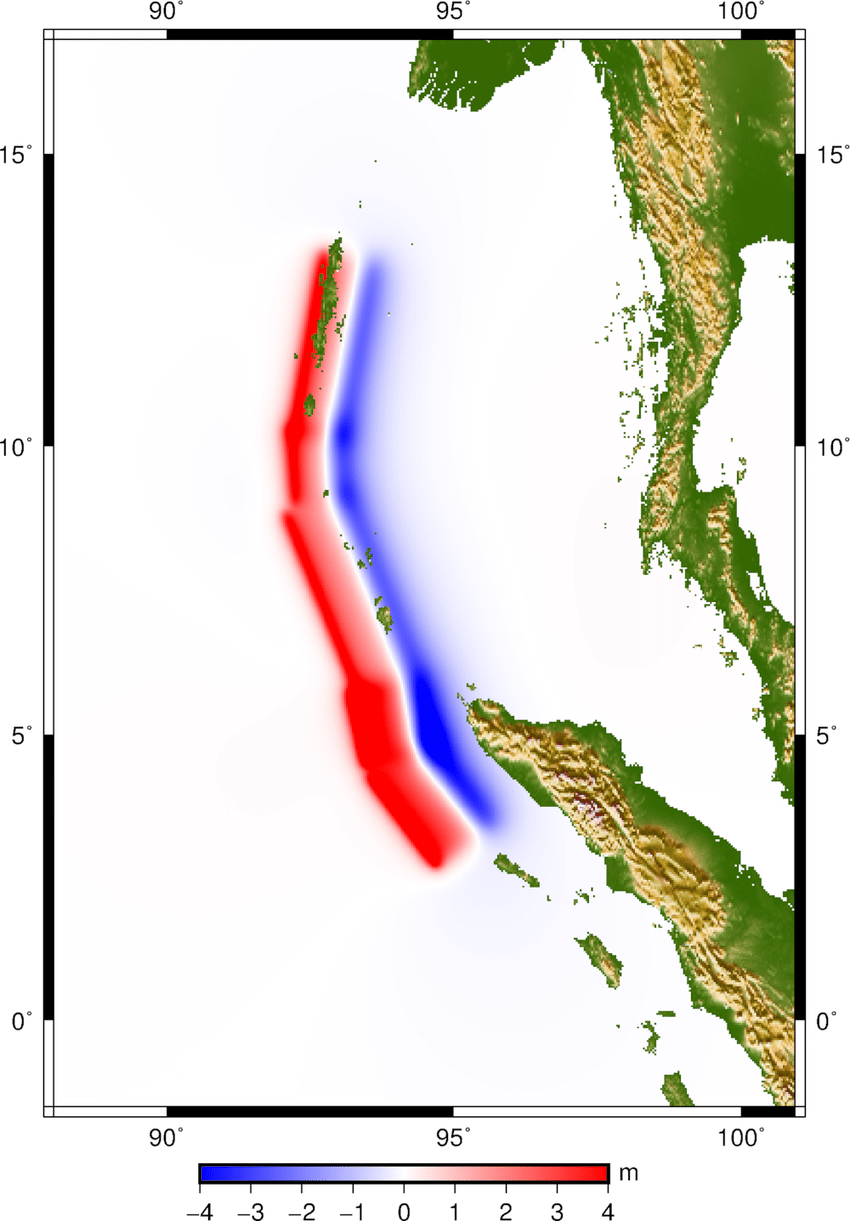
\includegraphics[width=0.35\textwidth]{./pics/water-surface.png}
            \caption{Earthquake generating a tsunami with $\lambda = 100\
            \text{km},\;\; a = 1\ \text{m}$ (found in \cite{graph_meter})}
        \end{figure}
    \end{frame}

    \begin{frame}
        \frametitle{2004 Tsunami: $\varepsilon=O\left(\delta^2\right)$}

        \begin{itemize}
            \item[$\circ$] $\varepsilon = \frac{a}{h_0}$ and $\delta =
                \frac{h_0}{\lambda}$ need to enter the regime
                $\varepsilon=O(\delta^2)$ for the KdV equation to become
                relevant
            \item[$\circ$] But also the geophysical scales need to be $\xi = O(1)$ and $\tau =
                O(1)$ for the KdV dynamics to become relevant, that is
                \begin{ceqn}
                \begin{align}
                    x = O\left(\varepsilon^{-1} \lambda \right)
                \end{align}
                \end{ceqn}
            \item[$\circ$] KdV dynamics is when the waves are ordered with the
                highest in front following an oscillatory tale
            \item[$\circ$] This happens because wave amplitude is proportional to
                wave speed
        \end{itemize}

    \end{frame}

    \begin{frame}
        \frametitle{2004 Tsunami: Regime of Validity}
        \begin{ceqn}
        \begin{align}
            \lambda = 100\ \text{km}\qquad a = 1\ \text{m}\nonumber
        \end{align}
        \end{ceqn}
        \begin{columns}
            \column{0.45\textwidth}
            Waves propagating westwards to India/Sri Lanka
            \begin{align}
            h_0 = 4\ \text{km} \Rightarrow
            \begin{cases}
                \varepsilon \simeq 25 \cdot 10^{-5}\\
                \delta \simeq 4\cdot 10^{-2}
            \end{cases}\nonumber
            \end{align}

            \column{0.45\textwidth}
            Waves propagating eastwards to Thailand
            \begin{align}
            h_0 = 1\ \text{km} \Rightarrow
            \begin{cases}
                \varepsilon \simeq 10^{-3}\\
                \delta \simeq 10^{-2}
            \end{cases}\nonumber
            \end{align}
        \end{columns}
        \vspace{0.5cm}
        \centering
        $\Rightarrow$ Both enter the regime $\varepsilon = O(\delta^2)$
    \end{frame}

    \begin{frame}
        \frametitle{2004 Tsunami: Regime of Validity}
        \begin{columns}
            \column{0.45\textwidth}
            Waves propagating westwards to India/Sri Lanka ($\simeq 1600\ \text{km}$)
            \begin{align}
                \begin{drcases}
                    \varepsilon \simeq 25\cdot 10^{-5}\\
                    \lambda = 100\text{km}
                \end{drcases}\Rightarrow\; x \simeq 4\cdot 10^{5}\ \text{km}\nonumber
            \end{align}

            \column{0.45\textwidth}
            Waves propagating eastwards to Thailand ($\simeq 700\ \text{km}$)
            \begin{align}
                \begin{drcases}
                    \varepsilon \simeq 10^{-3}\\
                    \lambda = 100\text{km}
                \end{drcases}\Rightarrow\; x \simeq 10^{5}\ \text{km}\nonumber
            \end{align}
        \end{columns}
        \vspace{0.5cm}
        \centering
        $\Rightarrow$ The propagation distance of the tsunami waves in both
        directions is not enough for KdV dynamics to take place.
    \end{frame}

    \begin{frame}{Bibliography}
        \printbibliography
    \end{frame}
\end{document}

